\documentclass[a4paper,12pt,preview]{report} %размер бумаги устанавливаем А4, шрифт 12пунктов
\usepackage[english,russian]{babel}%используем русский и английский языки с переносами 	
\usepackage[T2A]{fontenc}
\usepackage{changepage}
\usepackage{lipsum}
\usepackage{indentfirst}
\usepackage[labelsep=period]{caption}
\usepackage{amsmath}
\usepackage{textcomp}
%\usepackage{enumitem}
\usepackage[utf8]{inputenc}%включаем свою кодировку: koi8-r или utf8 в UNIX, cp1251 в Windows
\usepackage[english,russian]{babel}%используем русский и английский языки с переносами 	
\usepackage{amssymb,amsfonts,amsmath,mathtext,cite,enumerate,float} %подключаем нужные пакеты расширений
\usepackage{graphicx} %хотим вставлять в диплом рисунки?
\usepackage{ragged2e}
\usepackage{indentfirst}
\usepackage{titlesec}
\graphicspath{{images/}}%п\usepackage{trd}уть к рисункам

\makeatletter
\renewcommand{\@biblabel}[1]{#1.} % Заменяем библиографию с квадратных скобок на точку:
\makeatother

\usepackage{geometry} % Меняем поля страницы
\geometry{left=2cm}% левое поле
\geometry{right=1.5cm}% правое поле
\geometry{top=1cm}% верхнее поле
\geometry{bottom=2cm}% нижнее поле

\renewcommand{\theenumi}{\arabic{enumi}}% Меняем везде перечисления на цифра.цифра
\renewcommand{\labelenumi}{\arabic{enumi}}% Меняем везде перечисления на цифра.цифра
\renewcommand{\theenumii}{.\arabic{enumii}}% Меняем везде перечисления на цифра.цифра
\renewcommand{\labelenumii}{\arabic{enumi}.\arabic{enumii}.}% Меняем везде перечисления на цифра.цифра
\renewcommand{\theenumiii}{.\arabic{enumiii}}% Меняем везде перечисления на цифра.цифра
\renewcommand{\labelenumiii}{\arabic{enumi}.\arabic{enumii}.\arabic{enumiii}.}% Меняем везде перечисления на цифра.цифра

\newcommand{\doublerule}[1][.4pt]{%
	\noindent
	\makebox[0pt][l]{\rule[.7ex]{\linewidth}{#1}}%
	\rule[.3ex]{\linewidth}{#1}}



\titleformat{\chapter}[hang]
{\normalfont\huge\bfseries}{\thechapter.}{20pt}{}

\renewcommand*\thesection{\arabic{section}}

\newenvironment{boenumerate}
{\begin{enumerate}\renewcommand\labelenumi{\textbf\theenumi}}
	{\end{enumerate}}


\begin{document}
	
	\begin{center}
		Министерство образования и науки РФ \\
		Федеральное государственное автономное образовательное учреждение высшего профессионального образования <<НИТУ МИСиС>>\\
		Институт ИТАСУ\\
		Кафедра Инженерной кибернетики\\
	\end{center}
	
	
	\vfill
	
	\begin{center}
		\Large\textbf{Инструкция по эксплуатации системы\\ "Расписание занятий" \\
			по курсу <<Программная инженерия>>}
	\end{center}
	
	\vfill
	
	\begin{FlushRight}
		Выполнил\\
		Студент группы \\
		БПМ-16-2 \\
		Фадеев А.Ю. \\
		[\baselineskip]
		Проверил: \\
		Широков А.И. \\
		[9\baselineskip]
	\end{FlushRight}
	
	
	\begin{center}
		Москва 2020
	\end{center}
	
	\thispagestyle{empty}
	\newpage
	
	\tableofcontents
	\newpage
	
	\section{Общие положения.}
	
	Ниже приведена основная информация о проектируемом ПО.
	
	\subsection{Наименование системы.}
	Наименование системы - "Генератор фракталов"
	
	\subsection{Основание для проведения работ.}
	Основанием для данной работы служат требования учебной дисциплины "Программная инженерия"
	
	\subsection{Наименование организации -- заказчика и разработчика.}
	\subsubsection{Заказчик.}
	НИТУ «МИСиС», институт ИТАСУ, кафедра Инженерной кибернетики (доцент Широков А. И.).
	\subsubsection{Разработчик.}
	Исполнитель: Фадеев Александр, студент НИТУ «МИСиС», институт ИТАСУ, группа БПМ-16-2.
	
	\subsection{Цели, назначение и область использования системы.}
	Создание программной системы расписания занятий, удовлетворяющей требованиям к поставленной задаче.
		
	\subsection{Нормативные ссылки.}
	При техническом проектировании использовались следующие нормативно-технические документы:
	
	\begin{itemize}
		\item Техническое задание;
		\item Пояснительная записка к эскизному проекту;
		\item ГОСТ 19.102-77 (ЕСПД).
	\end{itemize}


		\section{Основные технические решения.}
	
	Готовое продукт должен подчиняться следующим алгоритмическим решениям и иметь следующие элементы интерфейса:
	
	\subsection{Разработка алгоритма решения задачи.}
	
	К заданному в \textit{"settings.txt"} полигону применяются преобразования подобия (являющиеся аффинными) заданное число итераций раз, полученное изображение визуализируется в основном окне.
	
	\subsection{Интерфейс.}
	
	Представляет собой окно визуализации и два дополнительных окна настроек, предоставляющих возможность посредством передвижения различных "ползунков" изменять те или иные характеристики основного изображения. Список регулируемых характеристик:
	
	Окно основных настроек:
	
	\begin{itemize}
		\item Масштаб.
		\item Число итераций применения преобразований подобия.
		\item Сдвиг центра координат по оси Х.
		\item Сдвиг центра координат по оси Y.
		\item Ширина изображения.
		\item Высота изображения.
		\item Режимы координатной сетки.
		\item Масштаб координатной сетки.
	\end{itemize}
	
	Окно дополнительных настроек:
	
	\begin{itemize}
		\item Цвет фона изображения.
		\item Цвет фрактала.
	\end{itemize}
	
	
	
	\section{Решение по режимам функционирования, работы системы.}
	
	будет функционировать в однопользовательском режиме, а также будет способна:
	
	\begin{itemize}
		\item Задания исходного множества и набора желаемых преобразований подобия.
		\item Визуализировать заданные фракталы.
		\item Сохранения изображения фрактала в файл.
	\end{itemize}
	
	\section{Решения по численности, квалификации и функциям персонала АС.}
	
	Указанные решения должны удовлетворять требованиям, приведенным в техническом задании на разработку системы.
	
	\section{Инструкция по взаимодействию с системой}
	
	\begin{enumerate}
		\item Для начала работы требуется разархивировать файл \textit{"fractals generator.rar"} с помощью, например, программы WinRar.
		
		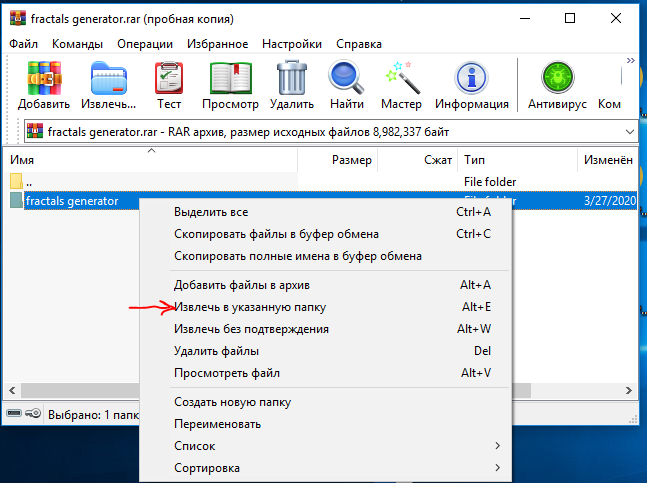
\includegraphics[scale=0.5]{Capture1.PNG}
		
		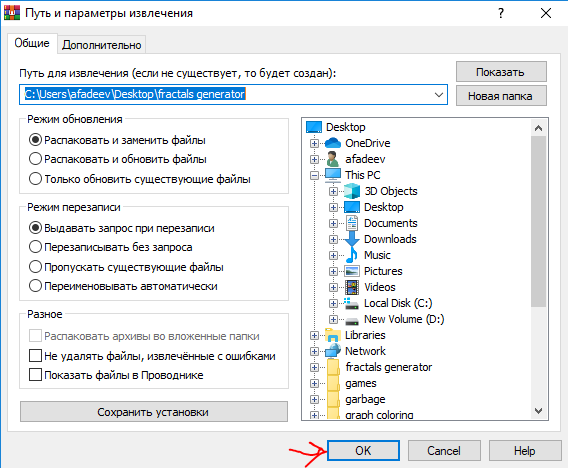
\includegraphics[scale=0.6]{Capture2.PNG}
		
		\item После этого требуется открыть директорию \textit{"fractals generator"} и запустить файл \textit{"fractals.exe"}.
		
		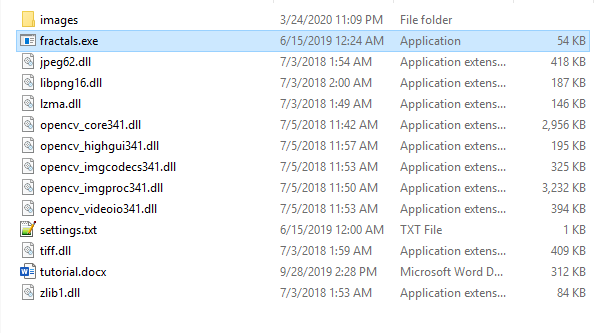
\includegraphics[scale=0.6]{Capture3.PNG}
		
		\item Должно появиться 3 окна:
		\begin{itemize}
			\item Окно визуализации.
			
			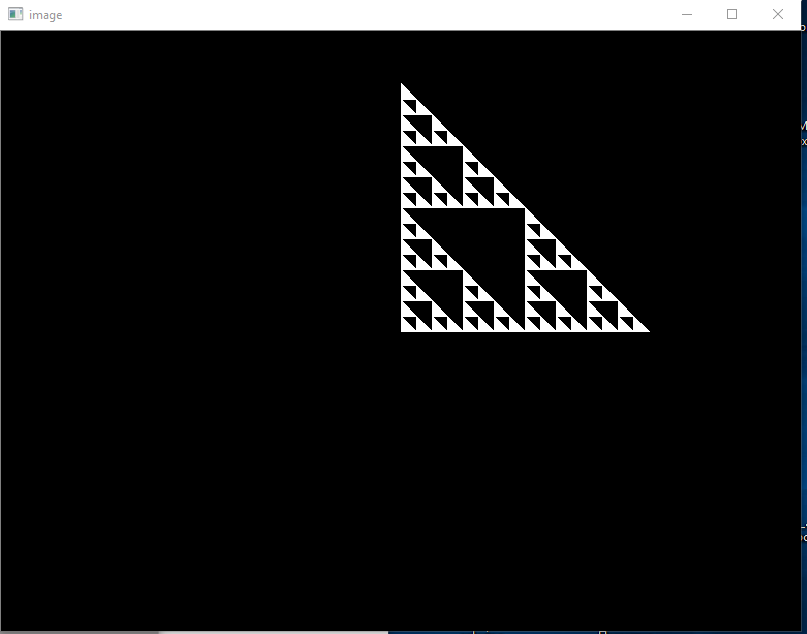
\includegraphics[scale=0.5]{Capture4.PNG}
			
			\item Окно настроек.
			
			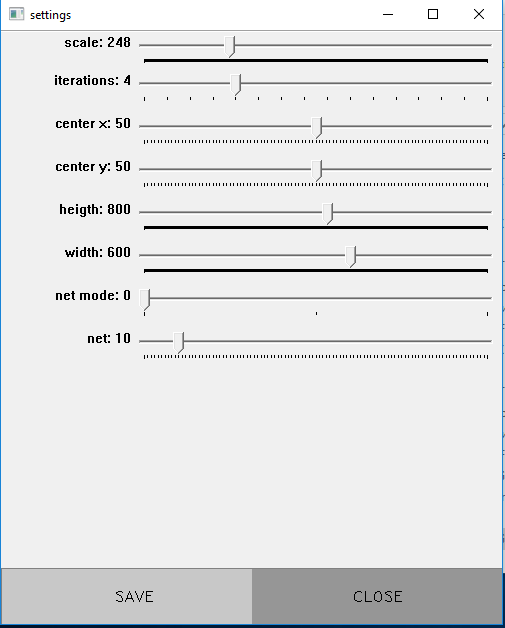
\includegraphics[scale=0.6]{Capture5.PNG}
			
			\item Окно дополнительных настроек.
			
			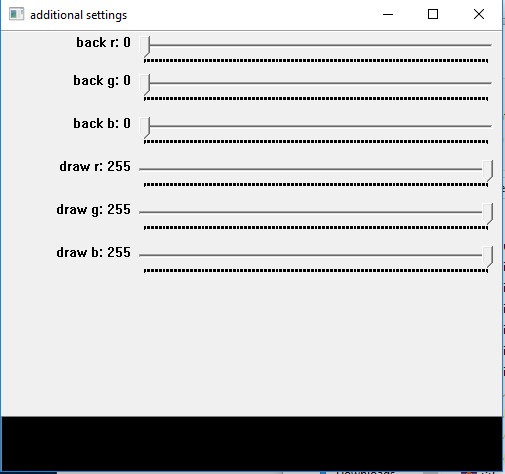
\includegraphics[scale=0.6]{Capture6.PNG}
		\end{itemize}
	
		Почти все возможные функции представлены на этих 3 экранах.
		
		\begin{enumerate}
			\item Задание изначального фрактала происходит через файл \textit{"settings.txt"}
			в соответствии с форматом, описанным в файле \textit{"tutorial.docx"}, которые находятся в той же директории.
			
			\item Визуализация происходит в одном из открывшихся окон.
			
			\item Сохранение полученного изображения происходит с помощью кнопки \textit{"SAVE"} окна основных настроек.
			
			\item Выход из программы осуществляется с помощью кнопки \textit{"CLOSE"} основного окна настроек.
			
			\item Изменения масштаба, параметров отрисовки координатной сетки, а также изменение количества итераций применения преобразований подобия осуществляется с помощью ползунков окна основных настроек.
			
			\item Изменение цвета изображения осуществляется с помощью ползунков окна дополнительных настроек.
			
			\item Примеры работы можно рассмотреть в документе \textit{"tutorial.docx"}.
			
		\end{enumerate}
		
		
	\end{enumerate}
	
\end{document}


